\chapter{Biological Background}

In order to better understand infectious diseases from a cell biological standpoint, this chapter reviews the current state of knowledge surrounding both bacterial and viral entry mechanisms. A sweeping overview of epidemology and pathogenesis for several specific bacterial (\textit{Bartonella henselae}, \textit{Brucella abortus}, \textit{Listeria monocytogenes}, \textit{Salmonella enterica} and \textit{Shigella flexneri}), as well as viral parasites (\textit{Adenovirus}, \textit{Rhinovirus} and \textit{Vaccinia virus}) is given and the chapter concludes with a look at RNA interference as this mechanism is a cornerstone of genome-wide knockdown experiments.

\section{Microbial Host-Cell Infection}

Multi-layered keratinized skin is impenetrable for almost all microbial parasites. Instead they either require breaches such as cuts, scratches, puncture wounds and arthropod bites, or environmental interfaces which offer less impervious protection. Examples include respiratory, gastrointestinal and urogenital tracts, which all contain segments where only a single layer of epithelial cells has to be overcome. Although often protected by chemical defense mechanisms (acidity of the stomach and urogenital tract, as well as microbicidal factors in mucous secretions in the respiratory tract and small intestine), combined with frequent flushing (urination, peristalsis and the coordinated beating of cilia), some microbes have adapted to survive these environments.

\newacronym{tir}{Tir}{translocated intimin receptor}
\newacronym{t3ss}{T3SS}{type III secretion system}

For extracellular pathogens to successfully colonize epithelial linings, they must avoid being removed by cleansing mechanisms of the host. Many bacteria accomplish this by expressing adhesins, protein complexes that recognize and bind to specific host-cell receptors, providing host and tissue tropism. Bacterial pili serve to extend reach and penetrate mucous secretions and therefore often carry adhesins. Enteropathogenic \textit{Escherichia coli} have extended this scheme by injecting their own receptor protein \revacr{tir} through the \revacr{t3ss} into the host cell to which it then attaches. This has the additional advantage that the intracellular domain of \gls{tir} can be used to modify host cell behavior \citep{Alberts2008}.

The outside of many epithelial barriers is covered in natural bacterial flora and crossing over into sterile cavities has the advantage of not having to compete with organisms well accustomed to that particular niche. Furthermore, intracellular pathogens are no longer accessible to antibodies and phagocytic cells and have a nutrient rich environment at their disposals. Mechanisms for entering host cells are described in the following sections.

\subsection{Viral Infection Mechanisms}

Viruses are entirely dependent on host-cell metabolism and machinery for their replication, making them obligately intracellular. The first step of any entering sequence is binding to the target surface. This can be mediated by attachment factors which simply serve to concentrate the virions on the cell membrane or by virus receptors, which additionally act as communicators between host and pathogen. Common attachment factors include glycosamminoglycan chains and sialic acids and are comparatively unspecific. Glycoprotein spikes on enveloped and capsid proteins of non-enveloped viruses provide host specificity by binding cellular receptors. Mostly these cellular receptors serve other purposes which are exploited for infection. Binding affinity for individual interactions may be weak but aggregation of multiple interactions provide virtually irreversible avidity \citep{Smith2012}.

For viral cell entry, different strategies exist. Enveloped viruses can either directly fuse with the plasma membrane (e.g. \gls{hiv}) or be endocytosed by the host cell (e.g. influenza), while non-enveloped viruses either create a pore and directly inject their genome into the cytosol (e.g. poliovirus) or are endocytosed (e.g. adenovirus). Endocytosis has major advantages over alternative strategies. Reaching its replicatory niche within the host cell is a difficult task for a micoorganism having no means of locomotion and hijacking the endocytic system solves this problem elegantly. Furthermore, maturation of endosomes provides precise environmental cues to the invader for triggering uncoating and release. Both fusion with the cell membrane and injection of viral material into the cytosol leaves back traces of infection to be detected by the immune system. Being completely engulfed by the host, virions leave back no telltale traces. Finally, lytic penetration techniques are not as problematic to the host if only applied inside an endosome.

Many endocytic viruses trigger clathrin-mediated, lipid-raft mediated or ma\-cro\-pi\-no\-cy\-tic mechanisms. The clathrin pathway is most commonly used (for example by rhinoviruses, some adenoviruses and influenza), while larger virions such as adeonvirus 3 or vaccinia virus initiate macropinocytosis, an actin dependent formation of a lamellipodium which folds back onto the plasma membrane, creating a macropinosome. Lipid raft dependent pathways are poorly understood. Simian virus 40 and polyomaviruses initiate cholesterol dependent formation of lipid rafts and trigger endocytic uptake by inducing plasma membrane curvature.

\begin{figure}
  \centering
  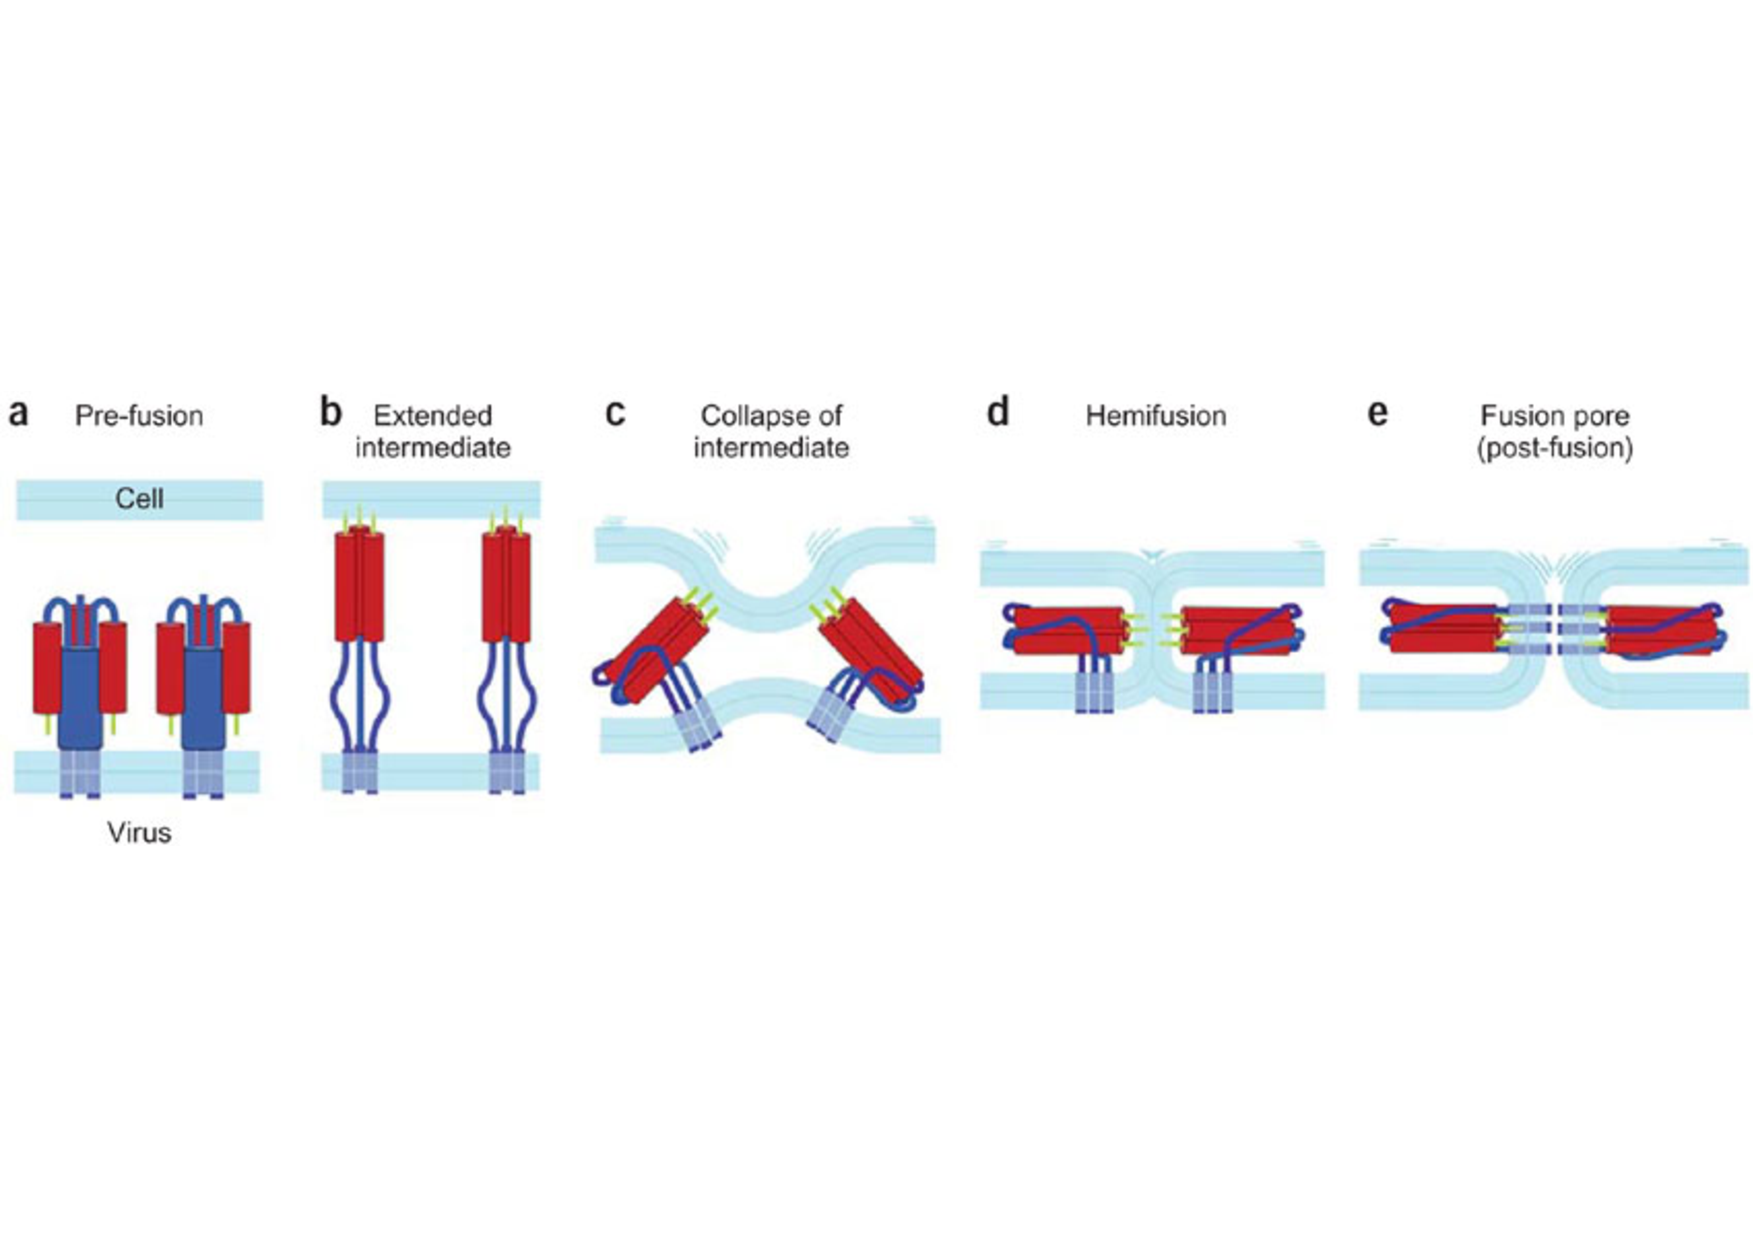
\includegraphics[width=0.95\textwidth]{viral-membrane-fusion}
  \caption[A generalized view of the steps necessary for viral--cellular membrane fusion]{A generalized view of the steps necessary for viral--cellular membrane fusion. (a) In pre-fusion conformation, fusion proteins have their hydrophobic fusion moieties tucked away. (b) Reacting to a trigger, such as low pH, the extended intermediate state is formed, characterized by exposed fusion sections, ready to interact with the target membrane. Conformational change in fusion proteins forces the two bilayers into close proximity, yielding first a collapsed intermediate state (c) and subsequently a state of hemifusion (d). Finally a fusion pore is formed (e), stabilized by the post-fusion conformation which is lower in energy than the pre-fusion state. \citep{Harrison2008}}
  \label{fig:viral-membrane-fusion}
\end{figure}

Upon endocytic uptake, viral pathogens need to uncoat and eject their genetic material into the cytosol, as soon as their replicatory niche is reached. Escape timing is a critical issue, as late endosomes finally turn into lysosomes, capable of digesting their contents. Many enveloped viruses employ fusion mechanisms, which can be classified as type I or type II. For both types, increasing acidity associated with endosome maturation, initiates membrane fusion. Type I fusion proteins are forced into a metastable conformation prior to being added to the viral envelope and low pH triggers a conformational change to a state of lower energy. The energy released is used to force the two membranes close together resulting in their fusion (see figure \ref{fig:viral-membrane-fusion}). In type II fusion proteins, the critical transformation is not a conformational change but one in quaternary structure.

\newacronym{er}{ER}{endoplasmic reticulum}
\newacronym{erad}{ERAD}{endoplasmic-reticulum-associated protein degradation}

Non enveloped viruses cannot fuse with host membranes and have developed alternative approaches such as lysis (e.g. adenovirus) or ejecting their genome through pore-forming complexes (e.g. reovirus). Polyomaviruses need to pass through the \gls{er} because they rely on \gls{er} localized proteins to uncoat their capsid. For export from the \gls{er} into the cytosol, they exploit the \gls{erad} pathway, which serves as export mechanism for misfolded proteins from the endoplasmic reticulum to be degraded by proteasomes.

\begin{table}
  \label{tab:activityTracking}
  \centering
  \caption{Tracking daily activities.}
  \footnotesize
  \begin{tabular}[c]{c|l|l|c|c}
    & Genome based class & Examples & Enveloped & Replication site\\
    \hline \multirow{2}{*}{\begin{sideways}DNA viruses\end{sideways}} &   
    Group I: dsDNA &
    Adenoviridae &
    no &\\
    \cline{2-5} &
    Group II: ssDNA(+) &
    Anelloviridae &
    no &\\
    \hline \multirow{3}{*}{\begin{sideways}RNA viruses\end{sideways}} &   
    Group III: dsRNA &
    Reoviridae &
    no &\\
    \cline{2-5} &
    Group IV: ssRNA(+) &
    Coronaviridae &
    yes &\\
    \cline{2-5} &
    Group V: ssRNA(-) &
    Paramyxoviridae &
    yes &\\
    \hline \multirow{2}{*}{\begin{sideways}Retroviruses\end{sideways}} &   
    Group VI: ssRNA(+)-RT &
    Lentivirus &
    yes &\\
    \cline{2-5} &
    Group VII: dsDNA-RT &
    Hepadnaviridae &
    yes &
  \end{tabular}
\end{table}


\subsection{Bacterial Entry Mechanisms}

Due to the much larger size of bacterial pathogens, endocytosis is not a feasible mechanism for entry. Phagocytosis, however can deal with particle uptake of this size magnitude. While phagocytosis is a function usually only available to macrophages, some bacteria have evolved mechanisms to induce phagocytosis in other cell types. Furthermore, species such as \textit{Mycobacterium tuberculosis} and \textit{Legionella pneumophila} targeting macrophages have to be able to escape phagosomes or deal with resisting digestion.

Two recurring patterns for inducing phagocytosis in non-phagocytic cells have been described: the zipper mechanism, found in \textit{Yersinia pseudotuberculosis} or \textit{Listeria monocytogenes} and the trigger mechanism used by \textit{Salmonella enterica} and \textit{Shigella flexneri}. Not all entry strategies can be assigned to these two classes and several additional, unrelated pathways have been described.

\begin{figure}
  \centering
  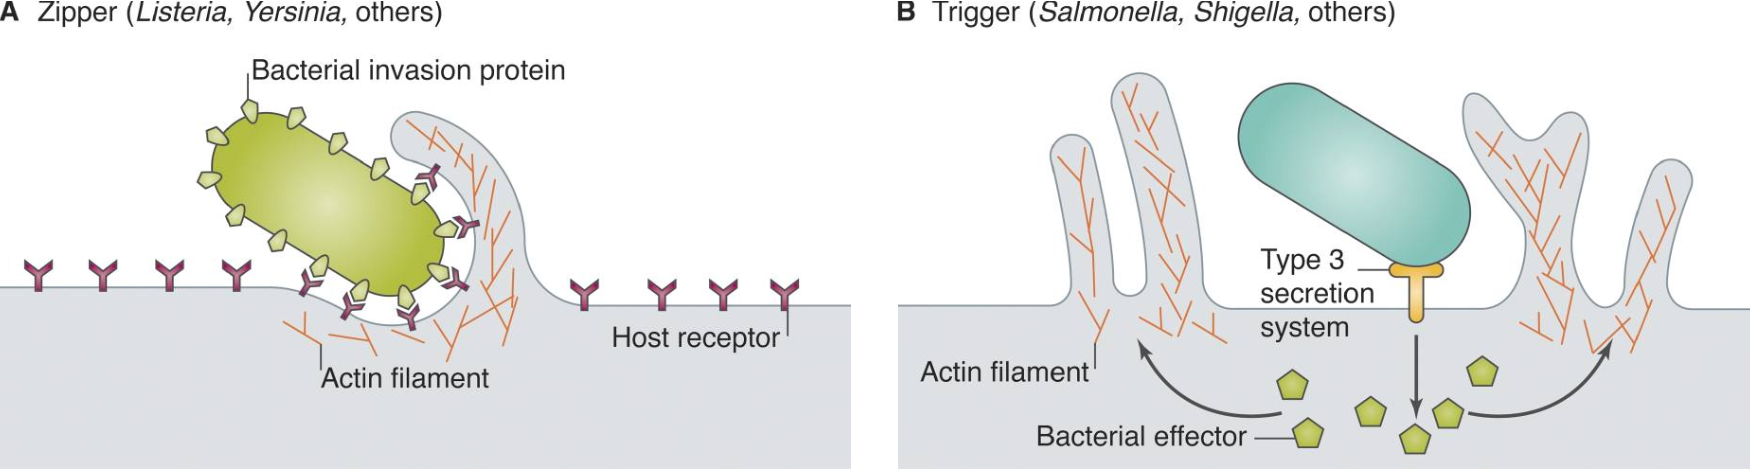
\includegraphics[width=0.95\textwidth]{zipper-trigger}
  \caption[Zipper and trigger mechanisms for bacterial host-cell entry]{Both the zipper (A) and trigger mechanisms (B) are actin dependent and lead to phagocytosis by usually non-phagocytic host cells. Zippering bacteria display an invasion protein on their surface that recruits actin filaments via a host receptor, while triggering bacteria inject an effector into the host cytosol via a type III secretion system leading to uptake. \citep{Haglund2011}}
  \label{fig:zipper-trigger}
\end{figure}

\newacronym{rac-1}{Rac1}{Ras-related C3 botulinum toxin substrate 1}
\newacronym{arp-2-3}{Arp2/3}{actin-related-protein 2 and 3}

\paragraph{Zipper Mechanism.}
The first step for zippering bacteria is binding to target cell receptors by expressing adhesins. \textit{Y. pseudotuberculosis} displays invasins on its cell surface, capable of interacting with \textbeta$_1$ integrins, while \textit{L. monocytogenes} uses internalin A, a protein that binds E-cadherin. In both settings, a downstream signaling cascade leads to actin polymerization via recruitment of an \revacr{arp-2-3} complex and \revacr{rac-1}, yielding a phagocytic cup.

Cadherin and integrins are usually involved in anchoring cell junctions and the host cell is fooled into thinking, a neighboring cell is initiating formation of such a junction. Responding by recruiting actin at the site of bacterial attachment to cover the surface of mistaken invasion proteins leads to engulfment and phagocytosis to the bacterium. This process incurs only modest cytoskeletal rearrangements. 

\newacronym{sip}{Sip}{\textit{Salmonella} invasion protein}
\newacronym{ipa}{Ipa}{\textit{Shigella} invasion plasmid antigen}

\paragraph{Trigger Mechanism.}
In case of the trigger mechanism, bacterial \gls{t3ss} weakly adhere to target cell receptors (CD44 for \textit{Shigella}) and effector molecules are injected into the host cytosol through a pore formed by \revacr{sip} or \revacr{ipa} proteins. These induce major actin rearrangements that result in localized ruffling of the plasma membrane and subsequent swallowing of the bacterium.

\newacronym{rac-1}{Rac1}{Ras-related C3 botulinum toxin substrate 1}
\newacronym{cdc-42}{Cdc42}{cell division control protein 42 homolog}

Early in \textit{Shigella} entry, VirA, secreted through the \gls{t3ss} causes local destabilization of microtubules by binding to \textalpha/\textbeta-tubulin heterodimers. This in turn stimulates \revacr{rac-1} activity, \revacr{cdc-42} recruitment and subsequent \gls{arp-2-3} activation leading to protrusions formed by actin filaments. \Gls{ipa}C recruits the Src tyrosine kinase further enhancing actin dynamics. Upon closing of the phagocytic pocket, the \gls{t3ss}-secreted protein \gls{ipa}A binds to vinculin and induces actin depolymerization.

\newacronym{sop-e}{SopE}{\textit{Salmonella} outer protein E}
\newacronym{spt-p}{SptP}{secreted effector protein}

\textit{Salmonella} inject the proteins \revacr{sop-e} and \revacr{spt-p}, an activator/inhibitor pair for the GTPase complex \gls{rac-1}/\gls{cdc-42}, into the host cell. First, GEF activity of \gls{sop-e} induces massive actin-rearrangements leading to membrane ruffling and facilitating phagocytosis, followed by GAP activity of \gls{spt-p}, restoring the inactive GDP state of \gls{rac-1}/\gls{cdc-42} and leading to actin depolymerization. \Gls{sop-e} is degraded more rapidly than \gls{spt-p}, enabling the invading pathogen to reversibly control the pathways exploited for entering.

\newacronym{t4ss}{T4SS}{type IV secretion system}

\paragraph{Other Entry Pathways.}
In addition to trigger and zipper type uptake, other atypical mechanisms exist. Host cell entry of \textit{Brucella abortus}, for example, has been described as invasome mediated \citep{Dehio2005}. In this actin dependent process, bacteria aggregate on the cell surface and trigger their engulfment by injecting bacterial effectors into the host via \gls{t4ss}. The internalized structure is called an invasome. So far, actin has always been the driving force behind internalization. Actin-independent uptake albeit rare, is possible as evidenced by \textit{Campylobacter jejuni}, which have evolved a microtubule dependent invasion strategy \citep{Kopecko2001}.

\subsection{Actin-based Intracellular Motility}

\section{Select Microbial Pathogens}

A total of 8 viral and bacterial pathogens were studied within the InfectX RTD project by SystemsX. This section shortly describes each organism in terms of microbiological features, pathogenesis, epidemiology and diseases caused in humans. The sections on bacteria are mostly based on \cite{Rolain2006} and for viruses, \cite{Craighead2000} was used as a basis.

\subsection{Bartonella Henselae}

\textit{Bartonella henselae} is a short, rod shaped, unflagellated proteobacterium, phylogenetically closely related to the genus \textit{Brucella}, presenting 94.4\% 16S rRNA gene sequence homology, compared with \textit{Brucella abortus}. The Gram-negative bacillus is a faculative anaerobic, intracellular parasite and was first described in 1992. Relatively harmelss for healthy humans, infections can become life threatening in immunocompromised patients, making the species an important opportunistic pathogen \citep{Anderson1997}.

\newacronym{csd}{CSD}{Cat Scratch Disease}

\paragraph{Diseases.}
In immunocompetent humans, infection with \textit{B. henselae} can lead to a condition known as \gls{csd}. As the name suggests, most patientent report being in contact with a cat and transmission often occurs through sratches and bites. Affecting primarily children and young adults (80\% are 21 or younger), the self limiting infection typically presents itself with lymphadenopathy. Most patients remain afebrile and do not report feeling ill, with low-grade fever and malaise shown in roughly 30\% of the cases. Recovery from uncomplicated \gls{csd} usually takes 2 to 6 months and requires no specific treatement.

Possible complications include Parinaud's oculoglandular syndrome (granulomatous conjunctivitis in one eye and parotid lymphadenitis on the same side), splenomegaly and hepatic or splenic abscesses, accompanied by fever, weight loss, fatigue and malaise. In 1 to 7\% of the cases, the disease spreads to the central nervous system, leading to encephalopathy, but recovery is usually rapid (within several weeks).

\newacronym{aids}{AIDS}{acquired immune deficiency syndrome}

Infections with \textit{B. henselae} tend to have more severe consequences for immunocompromised patients, such as bacillary angiomatosis, bacteremia and endocarditis. \Gls{aids} patients suffering from \gls{csd} usually experience severe, progressive disease with infection spreading systematically and without appropriate treatement, fatal outcome. \textit{Bartonella spp.} are the only prokaryotes known to be able to induce angiogenic tumors such as bacillary angiomas, which may involve skin, respiratory or gastrointestinal epithelia, hart, liver, spleen, bone marrow, muscles, or lymph nodes. Bacteremia may lead to inflamed heart valves, usually requiring endocarditic patients to have heart valve replacement surgery.

\newacronym{vegf}{VEGF}{vascular endothelial growth factor}
\newacronym{icam-1}{ICAM-1}{intercellular adhesion molecule 1}

\paragraph{Pathogenesis.}
\textit{B. henselae} are capable of intracellular growth in both epithelial cells, and erythrocytes. Bundle forming type IV pili are essential for binding to target cells, making them important virulence factors. Internalization into red blood cells may be spectrin mediated and the bacterial protein deformin may also be involved. Endothelial receptors involved include \gls{icam-1} uptake is either via endocytosis or by a unique cellular structure termed an invasome.

Vasculogenesis is induced though an increased production in \gls{vegf} by infected host cells. Currently it is poorly understood how the pathogen provokes overexpression but the mechanism has been determined to be protease sensitive.

\paragraph{Epidemiology.}
The role of cats and in particular kittens, as reservoirs to \textit{B. henselae} has been firmly estabished. Infected felines are asymptomatic and show no signs of illness. Cat fleas (\textit{Ctenocephalides felis}) serve as vectors to spread the bacteria among cats and have also been suspected of infecting humans. The main path of transmission to humans however, is through scratches and bites by infected cats. \textit{B. henselae} has also been found in ticks and tick bites prior to contraction of \gls{csd} have been reported.

In the United States, 24000 cases of \gls{csd} are reported yearly, yielding 2000 hospital admissions with an estimated health care cost of \$12 million. Children are more likely to be affected (80\%) and incidence is higher in males (60\%). The seasonal pattern (occurrences higher in fall/winter) is attributed to cat mating patterns, as well as pet acquisition fluctuations.

\subsection{Brucella Abortus}

\newacronym{lps}{LPS}{lipopolysaccharide}

The Danish physician David Bang first isolated \textit{Brucella abortus} in 1895 from cyetic cattle tissue, investigating a contagious disease causing abortions in cows. \textit{B. abortus} are small, unflagellated proteobacteria with a cell wall consisting of an outer layer of \gls{lps} (9 nm) and an inner layer of muramyl mucopeptide complexes (3--5 nm). The Gram-negative cocobacilli appear to have evolved from free-living, soil-dwelling species and are closely related to other human pathogens such as \textit{Bartonella} spp., based on 16S rRNA sequences. Brucella species were investigated for possible use as warfare agents in the mid 20th century by several armed forces. \citep{Atluri2011}

\paragraph{Diseases.}
Brucellosis is a human disease caused by several pathogenic \textit{Brucella} species, most importantly \textit{B. abortus}, \textit{B. melitensis}, \textit{B. canis} and \textit{B. suis}. Onset may be acute or insidious and due to protean symptoms, diagnosis based on clinical presentation alone is difficult. The febrile disease is generalized and may involve many parts of the body, including nervous, skeletal, gastrointestinal, cardiovascular, respiratory and genitourinary systems. Furthermore, as the bacteria spread to other reservoir hosts via their reproductive systems, persistence of infection is crucial to the pathogen and it comes as no surprise that brucellosis can manifest as a chronic disease in humans too.

Fever is the most consistent sign of \textit{Brucella} infection and depending on what specific organs are affected, further symptoms include asthenia, anorexia, nausea, malaise, arthritis, hepatomegaly, splenomegaly, epididymo-orchitis in males, and pulmonary manifestations such as bronchitis or pneumonia. A rare complication (less than 2\%), albeit the most lethal, is infective endocarditis. Invasion of the nervous system occurs in less than 5\% of cases and often results in meningitis or meningoencephalitis with good prognosis under antimicrobial treatment.

\paragraph{Pathogenesis.}
Host entry happens primarily via the digestive system but is also possible through the respiratory tract or skin lesions. On the gastrointestinal route, \textit{Brucella} spp. target Peyer's patches (lymphoid nodules localized towards the end of the small intestine) and must therefore pass through acidic conditions in the stomach. This is facilitated by expression of two ureases capable of hydrolyzing urea and producing a protective bicarbonate buffering system. When entering through the respiratory system, \textit{B. abortus} target alveolar macrophages which serve as access point to the lymphatic system therefore facilitating systematic spread.

\newacronym{tlr}{TLR}{toll-like receptor}
\newacronym{tir-1}{TIR}{toll-interleukin-1 receptor}

In order to persist at systemic sites, both active and passive mechanisms for evading the immune system are in place. \Gls{lps} of the outer cell wall disguises the bacteria from \glspl{tlr} and expression of two proteins containing \gls{tir-1} domains actively interferes with \gls{tlr} signaling.

\newacronym{ergic}{ERGIC}{ER-Golgi intermediate compartment}
\newacronym{cop-2}{COPII}{coat protein complex II, involved in anterograde \gls{er}--Golgi transport}

Uptake by macrophages happens via phagocytosis, which is either triggered by nonopsonized bacteria through a lipid raft mediated mechanism or by opsonisation. Although opsonin marked bacteria are 10-fold more likely to be ingested, the number of pathogens reaching their replicatory niche within the host cell is higher for nonopsonized bacteria. Maturation of early endosomes into lysosomes is important for successful infection as preventing acidification (through addition of bafilomycin A) or fusion with lysosomes (through suppression of the late-endosomal GTPase Rab7) interferes with bacterial replication. Nonopsonized bacteria finally become associated with rough ER and begin replication in ER derrived vacuoles within the \gls{ergic}. Blocking the small GTPase Sar1 inhibits intracellular replication by preventing acquisition of \gls{cop-2} by ER-exit vesicles and the small GTPase Rab2, involved in ER--cis-Golgi traffic, is required for maximal proliferation.

Despite multiplying intra-cellularly in high numbers, host cells are kept alive and are even able to replicate despite infection. Furthermore \textit{Brucella} species are able to interfere with apoptosis, maintaining their replicatory niche, protected from immune response.

\paragraph{Epidemiology.}
Preferred natural reservoir species for \textit{B. abortus} are cattle (\textit{Bos taurus} and \textit{Bos indicus}) and almost all parts of the world are affected. The disease exists in both domestic and wild animals and is most prevalent in Mediterranean countries, North Africa, throughout the Middle East, India, Central Asia, as well as South and Central America. Zoonosis most often occurs through ingestion if unpasteurized milk products but airborne transmission is also possible, putting professionals involved in animal husbandry at risk. Vertical transmission among reservoir hosts can occur through lactation and horizontal transmission is facilitated by mating and placental discharge associated with aborted gestation. Human-to-human transmission is rare (but has been suspected to be possible via sexual intercourse), making humans dead-end hosts. As opposed to \textit{Bartonella}, immunodeficient patients do not seem to be especially susceptible towards \textit{Brucella} infections.

\newacronym{who}{WHO}{World Health Organization}

Worldwide, an estimated 500000 new cases of brucellosis occur annually, making it one of the most prevalent zoonoses. Although usually susceptible to combined antibiotic therapies of at least two agents (usually a tetracycline antibiotic combined with an aminoglycoside or rifampin), untreated brucellosis leads to a high degree of morbidity, leading to being classified a neglected zoonosis by the \gls{who}.

\subsection{Listeria Monocytogenes}
\paragraph{Diseases.}
\paragraph{Pathogenesis.}
\paragraph{Epidemiology.}

\subsection{Salmonella Enterica}
\paragraph{Diseases.}
\paragraph{Pathogenesis.}
\paragraph{Epidemiology.}

\subsection{Shigella Flexneri}
\paragraph{Diseases.}
\paragraph{Pathogenesis.}
\paragraph{Epidemiology.}

\subsection{Adenovirus}
\paragraph{Diseases.}
\paragraph{Pathogenesis.}
\paragraph{Epidemiology.}

\subsection{Rhinoviruses}
\paragraph{Diseases.}
\paragraph{Pathogenesis.}
\paragraph{Epidemiology.}

\subsection{Vaccinia Virus}
\paragraph{Diseases.}
\paragraph{Pathogenesis.}
\paragraph{Epidemiology.}

\section{RNA Interference}
